\documentclass{thesis}

\title{Advanced Encryption Standard}

\subtitle{
    Cryptology Report
}

\author{
    Jiahui Dai (00153014)\\
    Yana Halamakh (00151596)\\
    Zeynep Melisa Akyol (00138182)
}

\supervisor{Prof. Katherine Roegner}


% Define acronyms
\newacronym{AES}{AES}{Advanced Encryption Standard}
\newacronym{VPN}{VPN}{virtual private network}
\makeglossaries


\begin{document}

% Cover Page (No page number)
\pagenumbering{gobble}  % Hide page numbering

% \input{coverpage}
\maketitle



% \thispagestyle{empty}
\section*{Affidavit}
\addcontentsline{toc}{section}{Affidavit}
\markright{Affidavit}

I certify that I have completed the work without outside help and without using sources other than those specified and that the work has not yet been submitted in the same or a similar form to any other examination authority and has been accepted by them as part of an examination. All statements that have been adopted literally or analogously are marked as such.

\vspace{3em}

Ingolstadt, \customdate\today
\newline
\hspace*{\fill}
\begin{tabular}{@{}l@{}}
\hline
\makebox[8cm]{Signature: Jiahui Dai (00153014)} \\[4cm] \hline
\makebox[8cm]{Signature: Yana Halamakh (00151596)} \\[4cm] \hline
\makebox[8cm]{Signature: Zeynep Melisa Akyol (00138182)} 
\end{tabular}
\newpage
\addcontentsline{toc}{section}{Acronyms}
\markright{Acronyms}
\printglossaries

% Abstract
\pagenumbering{roman}  
\setcounter{page}{1}  % Start from i
\section*{Abstract} %% <= Insert Title: Abstract vs. Summary
\addcontentsline{toc}{section}{Abstract}
\markright{Abstract}

This report delivers an in-depth exploration of the Advanced Encryption Standard (AES), 
a cornerstone in contemporary symmetric block cipher design and a vital element in today’s cryptographic frameworks. 
It starts by placing AES within its historical backdrop, 
shedding light on the shortcomings of its predecessor, 
the Data Encryption Standard (DES), 
which AES was explicitly developed to address. 
The document proceeds to unpack the inner workings of AES—detailing the mechanisms of both encryption and decryption, 
the structure of key expansion, and the underlying mathematics based on operations in Galois Fields. 
Core algorithmic steps are carefully explained, 
including SubBytes, ShiftRows, MixColumns, and AddRoundKey. 
To support practical understanding, the report features a working AES-128 implementation written in Python, thoroughly tested against the official NIST-provided test vectors to ensure accuracy. 
The report further explores real-world implementations of AES across domains such as wireless communication, 
secure cloud storage, and encrypted messaging, emphasising its broad adoption. 
It also offers a balanced assessment of AES’s strengths, 
such as its strong security guarantees and computational efficiency, 
while acknowledging specific practical issues like key distribution challenges and the absence of native authentication features. 
In its final analysis, 
the report examines how AES stands up to emerging quantum computing threats, 
concluding that the algorithm remains a relevant and reliable choice for modern and future cybersecurity demands.


% Table of Contents
\tableofcontents
\newpage

% Content
\pagenumbering{arabic}  
\setcounter{page}{1}
\section{Introduction}

\subsection{Background}

In today's connected digital world, cryptographic algorithms are implemented in every device and applied to every link to protect information in transmission and in storage.
Data security is a challenging issue that covers many areas including computer and communication.
There has been a rise of cyber attacks in gaining access to computers or computer networks, to gain information of private and sensitive data to gain information via communication channels or unsecure files \cite{csis2025significant}. 

Cryptology is the science of devising methods that allow information to be sent in a secure form in such a way that the only person able to retrieve the information is the recipient, through the use of algorithms. 
Data is exchanged while communicating from one system to another through the use of networks. 
It is important to encrypt the message so that unintended recipients (intruders) are unable to read the message as network security is highly based on cryptology  \cite{Bhanot_2015}.
% Modern cryptology aims to fulfil the following objectives \cite{Bhanot_2015}: 
% \begin{itemize}
%     \item \textbf{Confidentiality}: The information cannot be understood by anyone for whom it was unintended.
%     \item \textbf{integrity}: The information cannot be altered in storage or transit between sender and intended receiver without the alteration being detected.
%     \item \textbf{Non-repudiation}: The sender of the information cannot deny at a later stage that his or her intentions in the creation or transmission of the information.
%     \item \textbf{Authentication}: The sender and receiver can confirm each other's identity and the origin/destination of the information.
%     \item \textbf{Access Control}: Only authorised users can access data. 
% \end{itemize}

Over the past 50 years, the use of cryptographic tools have expanded dramatically, from limited environments like \gls{ATM} encryption to every digital application used today. 
\Gls{NIST} has played a unique leading role in developing critical standards \cite{chen2022cornerstone}:
\begin{itemize}
    \item \textbf{\Gls{DES}}: Developed in 1973 to protect computer data to allow for large-scale interoperability. \Gls{DES} uses a 64-bit block cipher with 56-bit key.
    \item \textbf{\Gls{AES}}: Developed in 1997 to superceeded \gls{DES}, with the use of 128-bit block cipher with three key length options: 128, 192, and 256 bits. 
    \item \textbf{Public-Key Cryptology}: Invented in 1976 to allow different parties to establish keys without protected channel and enabling the function of digital signatures. 
    \item \textbf{\Gls{PQC}}: Begun development in 2016 to develop quantum-resistant cryptography standards (i.e., \gls{PQC}) to provide security protection against quantum computers. As of writing this paper, \gls{NIST} have released the first three finalised Post-Quantum Encryption Standards \cite{nist2024postquantum}.
\end{itemize}


\subsection{Purpose of the paper}

The purpose of this paper is to provide a comprehensive overview of \gls{AES}, one of the most widly adopted encryption algorithms used to secure digital data.
The paper aims to explain the fundamental reasons for \gls{AES}'s development, the security challenges it addresses, and how it achieves strong encryption through its structured operations. 
By examining the internal workings of \gls{AES}, which includes its key expansion, substitution, permutation, and mixing steps, this paper seeks to demystify the encryption and decryption processes.
Furthermore, it explores the underlying mathematical principles that make \gls{AES} secure and resilient against cryptography attacks.
To reinforce understanding, the paper also includes simplified examples demonstrating how AES operates in practice. 
\newpage
\section{Advanced Encryption Standard (AES)}
\label{sec:purpose}

\subsection{What is AES?}

\textbf{\Glsentrylong{AES} (\gls{AES})} is the successor to \gls{DES}, with the algorithm developed by Vincent Rijmen and Joan Daeman (herein defined as Rijndael algorithm). 
It is a symmetric block cipher that can process data blocks of 128 bits, using cipher keys with lengths of 128, 192, and 256 bits \cite{NIST_AES}.
As the algorithm utilises different key lengths, they may be referred to as ``\gls{AES}-128'', ``\gls{AES}-192'' and ``\gls{AES}-256'' based on their key length, with ``\gls{AES}-128'' being adopted as the standard. 
Collectively, they will be referred as ``the \gls{AES} algorithm''.


\subsection{The role of AES in data security}

\noindent AES has been widely used in practice since it was standardised by NIST more than 20 years ago. 
It is implemented in protocols and products such as TLS, IPsec, IEEE 802.11i, SSH, 
WhatsApp, Signal, hard disk encryption tools, and many others. 
AES is the most widely used cipher in the world today and has strongly influenced modern block cipher design. 
Its design includes the wide trail strategy, which shows how the linear layer helps resist statistical attacks. 
Many successful modern block ciphers use design elements originally introduced in AES. 
Currently, no analytical attack that is significantly better than brute force is known on AES.\newline

\noindent In addition to its strong theoretical foundations, 
AES is highly efficient in both software and hardware. 
It supports high-throughput implementations and benefits from dedicated CPU instructions such as AES-NI (Advanced Encryption Standard New Instructions), 
accelerating performance in many modern systems. 
Even advanced cryptanalysis techniques, such as biclique attacks, 
provide only negligible improvements over brute-force approaches.\newline

\noindent Through this unique combination of robust security, practical efficiency, and broad adoption, 
AES plays a central role in safeguarding digital data across various applications and platforms.
\subsection{Security issues addressed}
\newpage
\section{How does AES work?}
\label{sec:how}

\subsection{Encryption and Decryption}

Encryption is the transformation of message bits (\textit{plaintext}) into unintelligible form (\textit{ciphertext}) using mathematical formulas (encryption algorithm).
Only the intended recipient with the decryption algorithm can decrypt the ciphertext to see the original message \cite{Devi_2019}.
Figure \ref{fig:encryption-process.png} shows the encryption and decryption process.

\begin{figure}[ht]
    \centering
    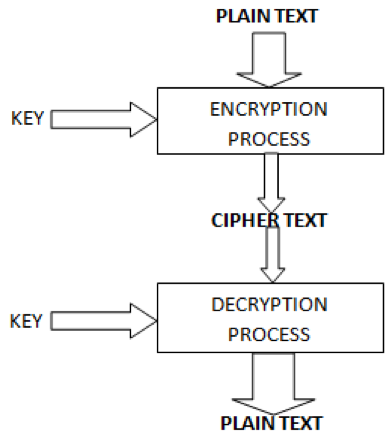
\includegraphics[width=.35\textwidth]{encryption-process.png}
    \caption{Encryption and decryption process \cite{Bhanot_2015}.}
    \label{fig:encryption-process.png}
\end{figure}


\subsubsection{Symmetric encryption}

Symmetric encryption algorithms use a single key that both the sender and recipient have.
This key is kept secret among sender and receiver so that no intruder can steal the data to be transferred by encrypting it  \cite{Bhanot_2015}.


\subsubsection{Asymmetric encryption}

Asymmetric encryption algorithm or public-key systems use two keys: a public key and a private key.
The public key is known to everyone while the private key is only used by the recipient of messages \cite{Bhanot_2015}.

Asymmetric encryption provides more security as compared to symmetric key encryption.
However, in case of encryption speed, symmetric encryption is on the lead \cite{Bhanot_2015}. 
\subsection{Stream and block ciphers}

Stream ciphers encrypt data one bit or one byte at a time.
They use a keystream, where each keystream bit is added to the plaintext individually \cite{Paar2024}.
An example would be the Caesar cipher, which substitutes one character with another individually.

Block ciphers process fixed-size blocks of data, with each block encrypted separately \cite{Paar2024}.

Stream ciphers are faster and more efficient than block ciphers as they encrypt one bit of data at a time rather than the entire blocks. 
Block ciphers can offer stronger security over stream ciphers, depending on its use \cite{Paar2024}. 
\subsection{AES algorithm workflow}

\Gls{AES} is a symmetric block cipher that operates on 128-bit blocks of data.
It processes these blocks in several rounds, with each round consisting of multiple layers that manipulate the data in specific ways. 
These layers introduce both \textit{confusion} and \textit{diffusion} to strengthen the encryption.

\subsubsection{Encryption process}

The AES structure consists of the following layers \cite{Paar2024}:
\begin{enumerate}
    \item \textbf{Key Addition Layer}:
    A 128-bit round key is \texttt{XOR} with the state, with round key generated in Key Expansion (Section~\ref{sec:key-expansion}).

    \item \textbf{Byte Substitution Layer (S-Box)}:
    Each byte of the state is non-linearly transformed using lookup tables. 
    This introduces confusion, ensuring that small changes in the input lead to significant, non-linear changes in the output.
    
    \item \textbf{Diffusion Layer}:
    This layer spreads the influence of each byte over the entire block. 
    It is divided into two sub-layers:
    \begin{enumerate}
        \item \textbf{\textsc{ShiftRow} Layer}: The rows of the state are shifted cyclically, which helps spread the data. %permutes the data on a byte level
        \item \textbf{\textsc{MixColumn} Layer}: This layer performs a matrix multiplication operation on the columns of the state, mixing the data across the block. % is a matrix operation which combines/mixes blocks of four bytes. 
    \end{enumerate}
\end{enumerate}

Each round, except the initial round, consists of all three layers. 
The initial round consists of only the Key Addition layer.
The final round omits the \textsc{MixColumn} transformation, making both encryption and decryption operations symmetric.
Figure \ref{fig:aes-block-diagram} shows the block diagram of AES encryption.

\begin{figure}[!ht]
    \centering
    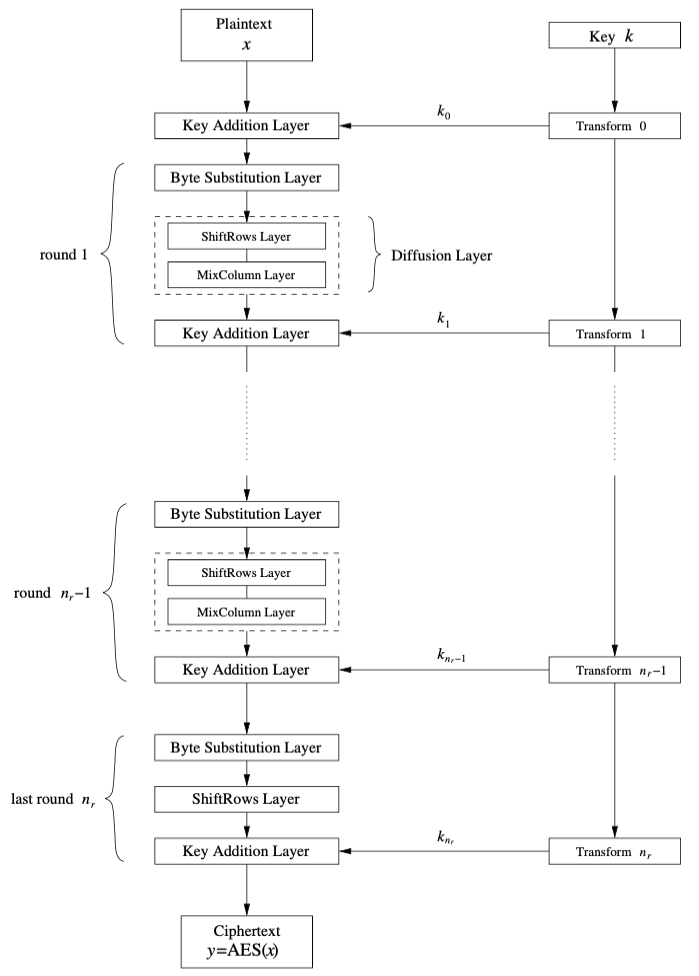
\includegraphics[width=.8\textwidth]{aes-block-diagram.png} % Adjust width as needed
    \caption{
        AES Encryption Block Diagram \cite{Paar2024}.
        The plaintext is denoted as $x$, the ciphertext as $y$, key as $k$, and the number of rounds as $n_r$.
    }
    \label{fig:aes-block-diagram}
\end{figure}


\subsubsection{Decryption process}
\label{sec:decryption}

AES decryption is the process of reversing encryption steps to retrieve the original plaintext from a given ciphertext. 
Since AES is a symmetric block cipher, it uses the same secret key for both encryption and decryption \cite{NIST_AES}.

The input data is handled in 128-bit blocks and processed through multiple transformation rounds. 
The number of rounds depends on the key size, as outlined in Table \ref{table:key-length-rounds}.

To decrypt, AES performs the inverse of each encryption step, but in reverse order. These inverse operations are:

\begin{enumerate}
    \item \textbf{AddRoundKey}: This step \texttt{XOR} the block with the corresponding round key. Since \texttt{XOR} is its own inverse, this operation is identical in both encryption and decryption.
    \item \textbf{InvMixColumns}: Reverses the mixing of bytes in each column. This step is skipped in the final round.
    \item \textbf{InvShiftRows}: Reverses the row shifts that were applied during encryption.
    \item \textbf{InvSubBytes}: Applies the inverse S-box substitution to each byte, undoing the non-linear transformation.
\end{enumerate}

Decryption starts by XORing the ciphertext with the final round key. 
Then, each round applies the inverse transformations using the appropriate round key from the key schedule. 
After all rounds are completed, the original plaintext is recovered.

\subsection{Key sizes and rounds}

In \gls{AES}, the block size is fixed at 128 bits, but the key size can vary between 128, 192, and 256 bits. 
The key length determines the number of rounds used in the encryption process, as outlined in Table \ref{table:key-length-rounds}.

\begin{table}[h]
    \centering
    \begin{tabular}{c|c}
        \textbf{Key length (bit)} & \textbf{\# rounds ($n_r$)} \\ 
        \hline
        128 & 10 \\  
        192 & 12 \\  
        256 & 14 \\  
    \end{tabular}
    \caption{Key lengths and number of rounds for AES \cite{Paar2024}.}
    \label{table:key-length-rounds}
\end{table}

\section{Why AES works?}
\label{sec:why}
\label{sec:math}

The 16-byte input $A_0, \dots, A_{15}$ is fed byte-wise into the S-Box in the Byte Substitution layer (Section~\ref{sec:SubBytes}).
The 16-byte output $B_0, \dots, B_{15}$ is permutated twice in the \textsc{ShiftRows} (Section~\ref{sec:ShiftRows}) and mixed by the \textsc{MixColumn} transformation (Section~\ref{sec:MixColumns}), both in the Diffusion layer.
Finally, the 128-bit subkey $k_i$ is \texttt{XOR} with the immediate result in the Key Addition layer (Section~\ref{sec:AddRoundKey}).
Figure~\ref{fig:aes-round-function} shows the graph of a single AES round. 

\begin{figure}[!ht]
    \centering
    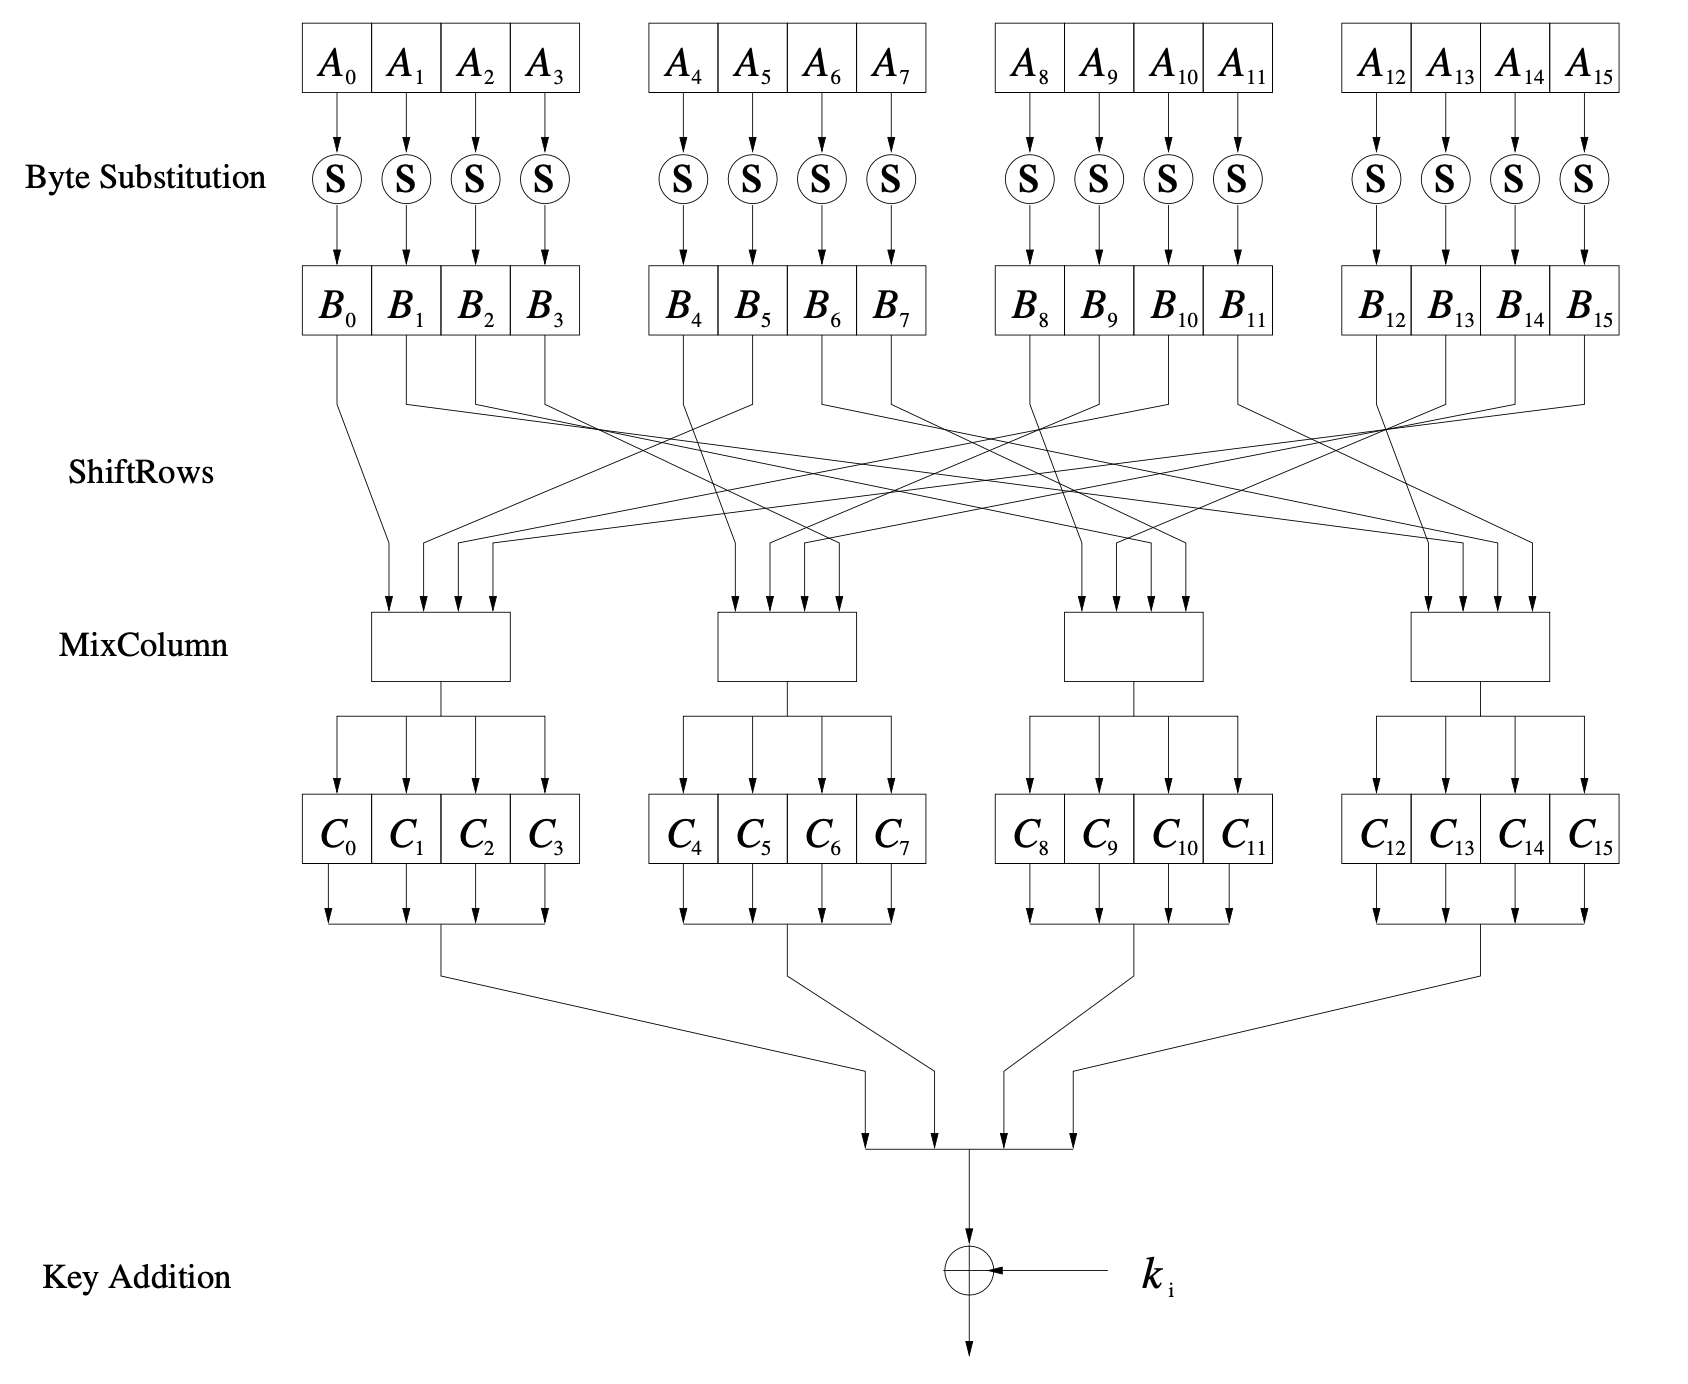
\includegraphics[width=\textwidth]{aes-round-function.png}
    \caption{
        AES round function for rounds $1, 2, \dots, n_r-1$ \cite{Paar2024}.
    }
    \label{fig:aes-round-function}
\end{figure}

The mathematical foundations discussed in subsequent subsections are based on the \gls{AES} specification published by \gls{NIST} \cite{NIST_AES} and the textbook by Paar and Pelzl \cite{Paar2024}.

\subsection{Mathematical Preliminaries}



\subsubsection{Addition}
\label{sec:addition}



\subsubsection{Multiplication}
\label{sec:multiplication}

\subsection{\textsc{SubBytes} transformation}
\label{sec:SubBytes}

The Byte Substitution layer can be viewed as a row of 16 parallel S-Boxes, each with 8 input and output bits (see Figure \ref{fig:aes-round-function}). 
Each state byte $A_i$ is replaced, i.e. substituted, by another byte $B_i$.

\begin{figure}[!ht] 
    \centering
    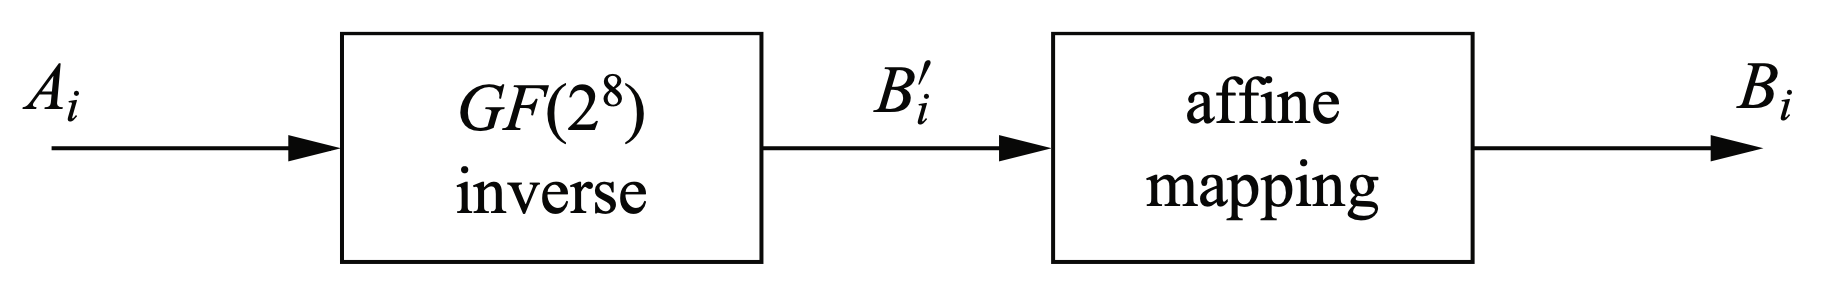
\includegraphics[width=.6\textwidth]{byte-substitution.png} 
    \caption{
        The two operations within the AES S-Box which computes the function $B_i = S(A_i)$ \cite{Paar2024}.
    }
    \label{fig:byte-substitution} 
\end{figure}

The \textsc{SubBytes} transformation is a non-linear byte substitution that operates independently on each byte of the state byte.
The S-Box is constructed by composing of two transformation:
\begin{enumerate}
    \item \textbf{Galois Field Inversion}: 
    Take the multiplicative inverse in the finite field $GF(2^8)$ and solve for ${B'}_i$ (Equation \ref{eq:gfi}), described in Section \ref{sec:multiplication}. 
    The element $\{00\}$ is mapped to itself.
    
    \begin{align}
        A_i \cdot {B'}_i &= 1 \mod P(x)
        \label{eq:gfi}
    \end{align}

    \item \textbf{Affine Mapping}:
    
    The following affine transformation (over $GF(2)$) is applied:
    \begin{align}
        b_i = {b'}_i \oplus {b'}_{(i+4 \mod 8)} \oplus {b'}_{(i+5 \mod 8)} \oplus {b'}_{(i+6 \mod 8)} \oplus {b'}_{(i+7 \mod 8)} \oplus c_i
    \end{align}
    for $0 \leq i \leq 8$, where $b_i$ is the $i$-th bit of the byte and $c_i$ is the $i$-th bit of a byte $c$ that is to be transformed.

    % Apply the following transformation with
    % each byte ${B'}_i$ is multiplied by a constant bit-matrix, followed by the addition of a constant 8-bit vector:
    % \begin{align}
    %     \begin{pmatrix}
    %         1 & 0 & 0 & 0 & 1 & 1 & 1 & 1\\
    %         1 & 1 & 0 & 0 & 0 & 1 & 1 & 1\\
    %         1 & 1 & 1 & 0 & 0 & 0 & 1 & 1\\
    %         1 & 1 & 1 & 1 & 0 & 0 & 0 & 1\\
    %         1 & 1 & 1 & 1 & 1 & 0 & 0 & 0\\
    %         0 & 1 & 1 & 1 & 1 & 1 & 0 & 0\\
    %         0 & 0 & 1 & 1 & 1 & 1 & 1 & 0\\
    %         0 & 0 & 0 & 1 & 1 & 1 & 1 & 1
    %     \end{pmatrix}
    %     \begin{pmatrix}
    %         {b'}_0\\
    %         {b'}_1\\
    %         {b'}_2\\
    %         {b'}_3\\
    %         {b'}_4\\
    %         {b'}_5\\
    %         {b'}_6\\
    %         {b'}_7
    %     \end{pmatrix}
    %     +
    %     \begin{pmatrix}
    %         1\\
    %         1\\
    %         0\\
    %         0\\
    %         0\\
    %         1\\
    %         1\\
    %         0
    %     \end{pmatrix}
    %     &\equiv
    %     \begin{pmatrix}
    %         b_0\\
    %         b_1\\
    %         b_2\\
    %         b_3\\
    %         b_4\\
    %         b_5\\
    %         b_6\\
    %         b_7
    %     \end{pmatrix}
    % \end{align}
    % where ${B'_i} = \left( {b'}_0, \dots, {b'}_7 \right)$ and $B_i = \left( b_0, \dots, b_7 \right)$
\end{enumerate}

% A lookup table for the \textsc{SubBytes} transformation can be generated by computing the substitution values for all possible two-digit hexadecimal inputs (i.e., 256 values from \texttt{00} to \texttt{FF}).
\textcolor{red}{insert lookup table}
\subsection{\textsc{ShiftRows}}

The \textsc{ShiftRows} transformation cyclincally shifts the second row of the state matrix three bytes to the right, the third row by two bytes to the right, and the forth row by one byte to the right (Eq. \ref{eq:ShiftRows}).
The first row is not changed.

The purpose of this is to increase the diffusion properties of AES.

\begin{equation}
    \begin{array}{c@{\quad \longrightarrow \quad}c}
        \begin{array}{|c|c|c|c|}
        \hline
        B_0 & B_4 & B_8 & B_{12} \\
        \hline
        B_1 & B_5 & B_9 & B_{13} \\
        \hline
        B_2 & B_6 & B_{10} & B_{14} \\
        \hline
        B_3 & B_7 & B_{11} & B_{15} \\
        \hline
        \end{array}
    &
    \begin{array}{|c|c|c|c|}
        \hline
        B_0 & B_4 & B_8 & B_{12} \\
        \hline
        B_5 & B_9 & B_{13} & B_1 \\
        \hline
        B_{10} & B_{14} & B_2 & B_6 \\
        \hline
        B_{15} & B_3 & B_7 & B_{11} \\
        \hline
        \end{array}
    \end{array}
    \label{eq:ShiftRows}
\end{equation}
\subsection{\textsc{MixColumns}}

The \textsc{MixColumn} transformation is a linear transformation which mixes each column of the state matrix. 
\begin{align}
    MixColumn(B) &= C\\
    \begin{pmatrix}
        02 & 03 & 01 & 01\\
        01 & 02 & 03 & 01\\
        01 & 01 & 02 & 03\\
        03 & 01 & 01 & 02
    \end{pmatrix}
    \cdot
    \begin{pmatrix}
        B_{0,c} \\
        B_{1,c} \\
        B_{2,c} \\
        B_{3,c} \\
    \end{pmatrix}
    &=
    \begin{pmatrix}
        C_{0,c} \\
        C_{1,c} \\
        C_{2,c} \\
        C_{3,c} \\
    \end{pmatrix}
\end{align}
for $0 \leq c \leq Nb$.
% with $B$ being the 16-byte input state after \texttt{ShiftRows} operation given in Equation \ref{} and C being the 16-byte output state.
% Each vector column of B is multiplied by a fixed $4 \times 4$ matrix (containing constant entries).

As a result of this multiplication, the four bytes in a column are replaced with the following
\begin{align}
    C_{0,c} & = (\{02\} * B_{0,c}) &&\oplus (\{03\} * B_{1,c}) &&\oplus B_{2,c} &&\oplus B_{3,c}\\
    C_{1,c} & = B_{0,c} &&\oplus (\{02\} * B_{1,c}) &&\oplus (\{03\} * B_{2,c}) &&\oplus B_{3,c}\\
    C_{2,c} & = B_{0,c}  &&\oplus B_{1,c} &&\oplus (\{02\} * B_{2,c}) &&\oplus (\{03\} * B_{3,c})\\
    C_{3,c} & = (\{03\} * B_{0,c}) &&\oplus B_{1,c} &&\oplus B_{2,c} &&\oplus (\{02\} * B_{3,c})
\end{align}

\subsection{\textsc{AddRoundKey} transformation}
\label{sec:AddRoundKey}

The \textsc{AddRoundKey} transformation combines the current state matrix with a round key derived from the key expansion process (Section \ref{sec:key-expansion}). 

This transformation operates by performing a bitwise \texttt{XOR} operation between each byte of the state matrix and the corresponding byte of the round key, represented as:
\begin{equation}
    C_{i,\text{out}} = C_{i,\text{in}} \oplus K_i
\end{equation}
where $ C_{i,\text{in}}$ and $C_{i,\text{out}}$ denote the input and output bytes of the state respectively, and $K_i$ represents the corresponding byte of the round key.

This step introduces key-dependent confusion into the encryption process, ensuring that the state is uniquely modified at each round based on the key material.
\subsection{Key Expansion (Key Schedule)}

\subsubsection*{Importance of Key Expansion in AES} 

The Advanced Encryption Standard (AES) heavily relies on the key expansion (or key schedule), 
a process that derives a series of round keys from the initial cipher key. 
This process ensures that each round uses a different key, 
greatly increasing the cipher's security. The key expansion process slightly differs 
based on the AES version (AES-128, AES-192, or AES-256), mainly in the number of rounds 
and the size of the key.

\subsubsection*{Main Algorithm of Key Expansion}

First, the initial key is loaded into the first $N_k$ words of the key schedule, where $N_k$ depends 
on the key size $K_{len}$ and the number of rounds $N_r$: ($K_{len}$, $N_r$) = (128, 10), (192, 12), and (256, 14) 
for AES-128, AES-192, and AES-256, respectively \cite{Key_Collisions} (shown in Figure~\ref{fig:key_comb}). AES requires $N_r+1$ round keys, each round key is 
128 bits (16 bytes) in size, equivalent to four words $N_b$ from the key schedule. The key schedule in 
response generates a total of $N_b$×($N_r+1$) words\cite{NIST_AES}. \newline

For example, for AES-192, the key schedule generates 52 words in the key expansion, which equals 208 bytes (4 \textit{bytes per word} × 52 \textit{words}).
13 round keys are then extracted from these words - one for each of the 12 rounds plus the initial key addition ($N_r$ + 1 = 13).

\begin{figure}[h] % 'h' means place the figure here if possible
    \centering
    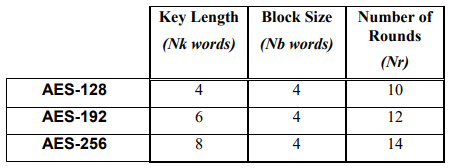
\includegraphics[width=.8\textwidth]{197_key_combinations.png} % Adjust width as needed
    \caption{
        Key-Block-Round Combinations \cite{Standards2001}
    }
    \label{fig:key_comb} % Reference this figure with \ref{fig:sample_image}
\end{figure}

Then, the remaining words are generated iteratively. For words at positions that are a multiple of $N_k$, a 
transformation is applied to the previous word w[i-1] before the \Gls{XOR}. This transformation consists of RotWord 
followed by SubWord, and the result is then XORed with a round constant Rcon[i], where:

\begin{enumerate}
    \item \textbf{RotWord}: A cyclic permutation that shifts the bytes in the 4-byte input word one position to the left. 
    \item \textbf{SubWord}: A substitution operation that applies SubBytes operation to a 4-byte input word. 
    \item \textbf{Round Constant (Rcon)}:  An \Gls{XOR} operation with a round-dependent constant RC, where each Rcon[i]
    has a structure (RC[i], 0x00, 0x00, 0x00) \cite{Standards2001}. 
\end{enumerate}

If the AES version is AES-256 ($N_k$ = 8) and i-4 is a multiple of $N_k$, the SubWord transformation is applied to the 
previous word (shown in Figure), but RotWord and Rcon are skipped. Otherwise, the new word is generated by XORing the previous word 
with the word $N_k$ positions earlier in the key schedule \cite{Standards2001}. 

\begin{figure}[h] % 'h' means place the figure here if possible
    \centering
    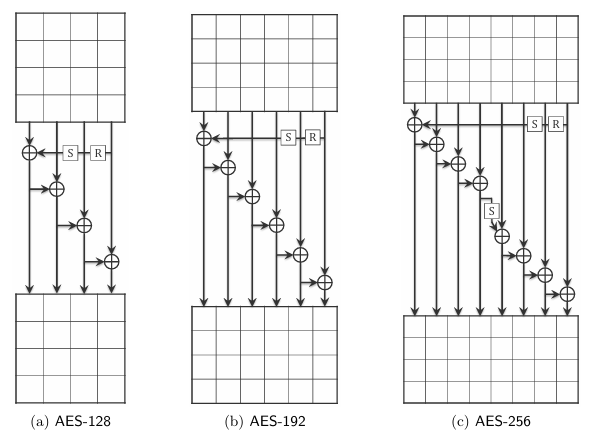
\includegraphics[width=.8\textwidth]{key_schedules.png} % Adjust width as needed
    \caption{
        Key schedules of AES-128, AES-192, and AES-256.The SubWord and
        RotWord functions are denoted by $S$ and $R$, respectively. Note that the round
        constant is not shown. \cite{Key_Collisions}
    }
    \label{fig:key_comb} % Reference this figure with \ref{fig:sample_image}
\end{figure}

\begin{figure}[h]
    \centering
    \includegraphics[width=.8\textwidth]{key_schedule-128.png}
    \caption{Key schedule for AES-128 \cite{Paar2024}.}
    \label{fig:key-schedule-128}
\end{figure}

\subsubsection*{Key Size and Security}

The key size directly impacts the security level of the algorithm, with 
longer keys providing higher security against brute force attacks. AES-128 offers sufficient security 
for most applications, but AES-192 and AES-256 are often preferred for applications requiring 
long-term security or protecting highly sensitive data. The increased number of rounds in AES-256 
further enhances its resistance against advanced cryptanalytic techniques.
\subsection{Security Properties}

Modes of operation define how a block cipher like AES is applied to variable-length data. 
Each mode introduces distinct security implications, 
including confidentiality, error propagation, resistance to structural analysis, 
and resilience against future threats such as quantum computing.

\noindent The security of a mode depends not only on AES itself but also on how the blocks are processed. 
For instance:

\begin{itemize}
    \item \textbf{\Gls{ECB} Mode} encrypts each block independently, leading to pattern leakage. Identical plaintext blocks produce identical ciphertexts, compromising confidentiality, especially in structured data like images.
    
    \item \textbf{\Gls{CBC} Mode} introduces randomisation through an \Gls{IV}, ensuring that identical messages yield different ciphertexts. However, encryption is inherently sequential and more sensitive to bit-flip propagation.
    
    \item \textbf{\Gls{CFB} and \Gls{OFB} Modes} convert the block cipher into a stream cipher. OFB offers better error isolation, while CFB is self-synchronising but more susceptible to feedback-based error propagation.
    
    \item \textbf{\Gls{CTR} Mode} enables full parallelism and random access by encrypting incrementing counters. It avoids feedback loops and supports high-throughput use cases, making it robust in environments requiring speed and scalability.
    
    \item \textbf{\Gls{XTS}-AES} is optimised explicitly for disk encryption. It uses a tweakable block cipher based on sector position to ensure that the same data encrypted at different locations yields different ciphertexts, offering strong structural and positional integrity.
\end{itemize}

With the anticipated rise of quantum computing, 
AES modes must also be evaluated under quantum threat models. 
Grover’s algorithm reduces brute-force complexity from $2^k$ to approximately $2^{k/2}$. \newline

Jang et al.\cite{Jang2025} present refined circuit depth and gate count estimates under realistic quantum constraints. 
Their study indicates the following effective quantum security levels:

\begin{itemize}
    \item AES-128: $2^{156.26}$
    \item AES-192: $2^{221.58}$
    \item AES-256: $2^{286.07}$
\end{itemize} 

These values, derived using optimised Grover-based search circuits, 
are well above the estimated practical capabilities of near-term quantum computers\cite{Jang2025}. \newline

Importantly, parallelisable modes like CTR and XTS are more amenable to low-depth quantum circuit implementations. 
Their compatibility with constraints such as NIST’s \texttt{MAXDEPTH} parameter makes them promising candidates for quantum-resilient applications\cite{Jang2025}.

\begin{table}[h]
\centering
\resizebox{\textwidth}{!}{%
\begin{tabular}{|l|c|c|c|l|}
\hline
\textbf{Mode} & \textbf{Parallel} & \textbf{Error Propagation} & \textbf{Random Access} & \textbf{Best Use Case} \\
\hline
\Gls{ECB} & Yes & None & Yes & Toy cases, testing only \\
\Gls{CBC} & No (Enc) / Yes (Dec) & Yes(next block) & No & File encryption \\
\Gls{CFB} & No & Yes(next block) & No & Streaming data with feedback \\
\Gls{OFB} & Yes & None & No & Resilient byte-wise streaming \\
\Gls{CTR} & Yes & None & Yes & High-throughput systems \\
\Gls{XTS} & Yes & None & Yes & Secure disk encryption \\
\hline
\end{tabular}%
}
\caption{Security characteristics of AES modes of operation.}
\end{table}
\newpage


\section{Practical demonstration of AES}
\label{sec:example}

\subsection{Implementation details}

Building on the mathematical foundation outlined in Section~\ref{sec:why}, the AES algorithm was implemented in Python to demonstrate its practical application.
This implementation supports only AES-128, and require both the encryption key and input data to be provided in hexadecimal format. 
The complete source code is provided in Appendix~\ref{appendix:code}.

The implementation is structured across three Python modules: \texttt{functions.py}, \texttt{bin\_math.py}, and \texttt{aes.py}, each responsible for a specific aspect of the algorithm.

The \texttt{functions.py} module (see Python Code~\ref{lst:fxns}) contains general-purpose helper functions used throughout the AES implementation. 
These functions include:
\begin{itemize}
    \item \texttt{process\_str(string)}: Removes all whitespace from a given string.
    \item \texttt{process\_key(key, Nk=4)}: Processes a hexadecimal key string into a $4\times4$ \texttt{NumPy} array of bytes.
    \item \texttt{process\_input\_hex(input\_hex)}: Processes a hexadecimal input (e.g., plaintext or ciphertext) into a $4\times4$ AES state matrix.
    \item \texttt{bytes\_to\_word(bytes\_list)}: Converts a list of 4 bytes into a 32-bit word.
    \item \texttt{word\_to\_bytes(word)}: Converts a 32-bit word into a list of 4 bytes.
    \item \texttt{state\_to\_hex(state)}: Converts a $4\times4$ AES state matrix into a hexadecimal string representation.
\end{itemize}

The \texttt{bin\_math.py} module (see Python Code~\ref{lst:bin-math}) implements the arithmetic operations required for AES's finite field calculations. 
This module includes:
\begin{itemize}
    \item \texttt{gf\_mult(a, b)}: Performs Galois Field multiplication of two bytes, as explained in Section~\ref{sec:multiplication}.
    \item \texttt{generate\_gf(primitive\_element)}: Constructs the extension field GF($2^8$) using a given primitive element, as described in Section~\ref{sec:multiplication}.
\end{itemize}

The core AES encryption logic is implemented in the \texttt{aes.py} module (see Python Code~\ref{lst:aes-impl}). 
This module includes the main algorithmic transformations and key scheduling logic, as described below:
\begin{itemize}
    \item \texttt{load\_properties(key\_length)}: Loads AES parameters such as the number of rounds based on the specified key length.
    \item \texttt{generate\_sbox()}: Generates the AES S-Box used in the \textsc{SubBytes} step (see Section~\ref{sec:SubBytes}).
    \item \texttt{generate\_rc(Nr=10)}: Produces a list of round constants used in the key expansion process (see Section~\ref{sec:key-expansion}).
    \item \texttt{g(word, rc)}: Implements the transformation function used during key expansion (see Section~\ref{sec:key-expansion}).
    \item \texttt{KeyExpansion(key, Nb=4, Nk=4, Nr=10)}: Performs AES key expansion to generate round keys (see Section~\ref{sec:key-expansion}).
    \item \texttt{enter\_key(key)}: Prepares and expands the encryption key by processing it and initializing the key expansion.
    \item \texttt{SubBytes(state)}: Performs the \textsc{SubBytes} transformation to the AES state (see Section~\ref{sec:SubBytes}).
    \item \texttt{ShiftRows(state)}: Performs the \textsc{ShiftRows} transformation (see Section~\ref{sec:ShiftRows}).
    \item \texttt{MixColumns(state)}: Performs the MixColumns transformation (see Section~\ref{sec:MixColumns}).
    \item \texttt{AddRoundKey(state, keys)}: Adds the round key to the current state using \texttt{XOR} (see Section~\ref{sec:AddRoundKey}).
    \item \texttt{encrypt(input\_)}: Executes the full AES encryption procedure on the given input.
\end{itemize}
\subsection{Results and Analysis}

The AES implementation was tested using the script aes.py with a predefined key and plaintext input. 
The parameters used for this test are detailed below:

{\ttfamily
\begin{tabular}{ll}
    key: & 000102030405060708090a0b0c0d0e0f\\
    plaintext: & 00112233445566778899aabbccddeeff
\end{tabular}
}

Upon execution, the resulting ciphertext output was:

{\ttfamily
\begin{tabular}{ll}
    ciphertext: & 69C4E0D86A7B0430D8CDB78070B4C55A
\end{tabular}
}

This output matches the expected result defined in the official \gls{AES} specification published by the \gls{NIST} \cite{NIST_AES}.
The consistency of this result validates the correctness of the \gls{AES} encryption implementation in \texttt{aes.py}.

\subsection{Possible future work}

Future work could focus on extending the current implementation to include AES-192 and AES-256, which would involve handling their respective key lengths and more complex key expansion procedures. 
Additionally, implementing the decryption process would provide a complete encryption-decryption cycle, enabling full functionality of the AES algorithm. 
Another potential enhancement is to allow input keys and plaintext data in formats other than hexadecimal, such as ASCII or binary, by incorporating automatic conversion methods. 
Finally, a comparative analysis of runtime complexity and execution time for encryption and decryption across AES-128, AES-192, and AES-256 could provide valuable insights into the performance and efficiency trade-offs among these variants.
\newpage
\section{Applications and Limitations}

\subsection{Common use case}
\subsection{Strengths}
\subsection{Limitations and considerations:}

Despite its many strengths, using AES in practice has several important challenges that can affect security 
and effectiveness of cryptographic solutions.

\subsubsection*{Key Management}

No symmetric cipher, including AES, can guarantee security if key management practices are poor. The entire 
method fundamentally depends on the secrecy, integrity, and lifecycle management of keys. Secure generation, 
distribution, rotation, storage (often using physical security modules), and destruction are critical.

Regardless of AES's mathematical strength, mistakes — such as using weak keys, allowing key reuse, failing to 
rotate compromised keys, or transmitting keys over insecure channels—can undermine the confidentiality of 
encrypted data.

\subsubsection*{Implementation Vulnerabilities}

AES's theoretical resilience is not immune to practical attacks targeting its real-world implementation. 
Side-channel attacks—such as timing, cache, power consumption, or electromagnetic radiation analysis—can 
reveal key material if the implementation is not carefully handled. Mitigating these risks requires additional 
programming practices like constant-time implementations or mathematically secure curves.

\subsubsection*{Lack of Built-In Authentication}
AES offers confidentiality, but it does not include a way to verify that the encrypted data hasn't been tampered 
with. Data integrity and authenticity must be added using \Gls{MAC}s or by adopting combined authenticated encryption 
modes like \Gls{GCM} or \Gls{CCM} \cite{rfc4494}. Neglecting to supplement basic AES with integrity checks can expose the system to forgery 
and modification attacks.
\section{Conclusion}





\hrule

% \section{Introduction to Cryptography}

\subsection{Why Do We Need Encryption?}

With the development of technology, there are more ways of communication. Many years ago, people used Morse code; now, people write text messages on smartphones through apps that claim to provide end-to-end encryption. But where does this need come from, and why do we need encryption?

Through encryption, we secure our privacy, prevent unauthorized access to our lives, protect government systems against attacks, and, for many companies, keep corporate secrets safe from competitors. Unauthorized listening to private communication is known as \textit{eavesdropping}~\cite{Paar2024}.

\subsection{Symmetric and Asymmetric Encryption}

Symmetric encryption uses one key to encrypt and decrypt data. Before communication, the sender and receiver must securely share the key~\cite{Paar2024}.

Asymmetric encryption uses a pair of keys: a public key and a private key. The public key is shared with everyone, while the private key is unique to the receiver. Thus, the public key encrypts, and the private key decrypts~\cite{Paar2024}.

AES and DES are examples of symmetric encryption, whereas RSA is an example of asymmetric encryption~\cite{Paar2024}.

The main difference between symmetric and asymmetric encryption is that symmetric encryption is faster since it uses the same key for both encryption and decryption. Asymmetric encryption is slower but solves the key exchange problem. Therefore, they are often combined: asymmetric encryption securely shares a key, and symmetric encryption is used for fast communication~\cite{Paar2024}.
% \section{Definition and Comparison to Stream Ciphers}

In symmetric cryptography, block ciphers and stream ciphers are two main types.

Stream ciphers encrypt data one bit or one byte at a time. 
They use a \textit{keystream}, where each keystream bit is added to a plaintext bit individually.

\begin{figure}[h] % 'h' means place the figure here if possible
    \centering
    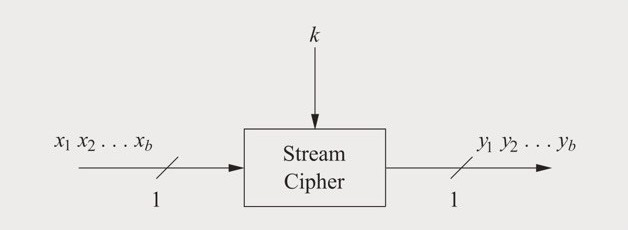
\includegraphics[width=.7\textwidth]{streamc.jpeg}
    \caption{Stream cipher operation}
    \label{fig:stream_cipher}
\end{figure}

Block ciphers process fixed-size blocks of data, with each block encrypted separately.

\begin{figure}[h]
    \centering
    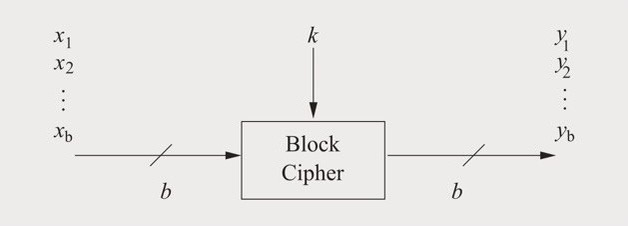
\includegraphics[width=0.7\textwidth]{blockc.jpeg}
    \caption{Block cipher operation}
    \label{fig:block_cipher}
\end{figure}



\begin{table}[h]
\centering
\begin{tabular}{|c|c|}
\hline
\textbf{Block Cipher} & \textbf{Stream Cipher} \\
\hline
Encrypts chunks (blocks) & Encrypts continuously, bit by bit \\
\hline
Offers more security when used properly & Can be faster and have less delay \\
\hline
\end{tabular}
\caption{Comparison between block cipher and stream cipher.}
\label{tab:block_vs_stream}
\end{table}
% \section{Overview}

The \textbf{Advance Encryption Standard (AES)}, also known as the Rijndael, is the most widely used symmetric cipher today.
It is mandated by several industry standards and incorporated into numerous commercial systems. 
Examples include the Wi-Fi encryption standard IEEE 802.11i, the secure shell network protocol SSH (Secure Shell), and numerous security products around the world. 

AES was developed to replace Data Encryption Standard (DES), becoming the new standard for encryption.
% DES is known to not be very efficient for software implementions and it uses a short block size of 64 bits, which is a drawback in certain applications. 
% For example, building a hash function from a block cipher. 


\subsection{General Structure of AES}

AES operates on 128-bit blocks of data, referred to as the state of the algorithm.
It processes these blocks in several rounds, with each round consisting of multiple layers that manipulate the data in specific ways. 
These layers introduce both \textit{confusion} and \textit{diffusion} to strengthen the encryption.

The AES structure consists of the following layers:
\begin{enumerate}
    \item \textbf{Key Addition Layer}:
    A 128-bit round key is XORed with the state. 
    % This adds the key information to the data at each round. 

    \item \textbf{Byte Substitution Layer (S-Box)}:
    Each byte of the state is non-linearly transformed using lookup tables. 
    This introduces confusion, ensuring that small changes in the input lead to significant, non-linear changes in the output.
    
    \item \textbf{Diffusion Layer}:
    This layer spreads the influence of each byte over the entire block. 
    It is divided into two sub-layers:
    \begin{enumerate}
        \item \textbf{ShiftRow Layer}: The rows of the state are shifted cyclically, which helps spread the data. %permutes the data on a byte level
        \item \textbf{MixColumn Layer}: : This layer performs a matrix multiplication operation on the columns of the state, mixing the data across the block. % is a matrix operation which combines/mixes blocks of four bytes. 
    \end{enumerate}
\end{enumerate}

Each round, except the first, consists of all three layers. 
The final round omits the \textsc{MixColumn} transformation, making both encryption and decryption operations symmetric.

Figure \ref{fig:aes-block-diagram} shows the block diagram of AES encryption.

\begin{figure}[h] % 'h' means place the figure here if possible
    \centering
    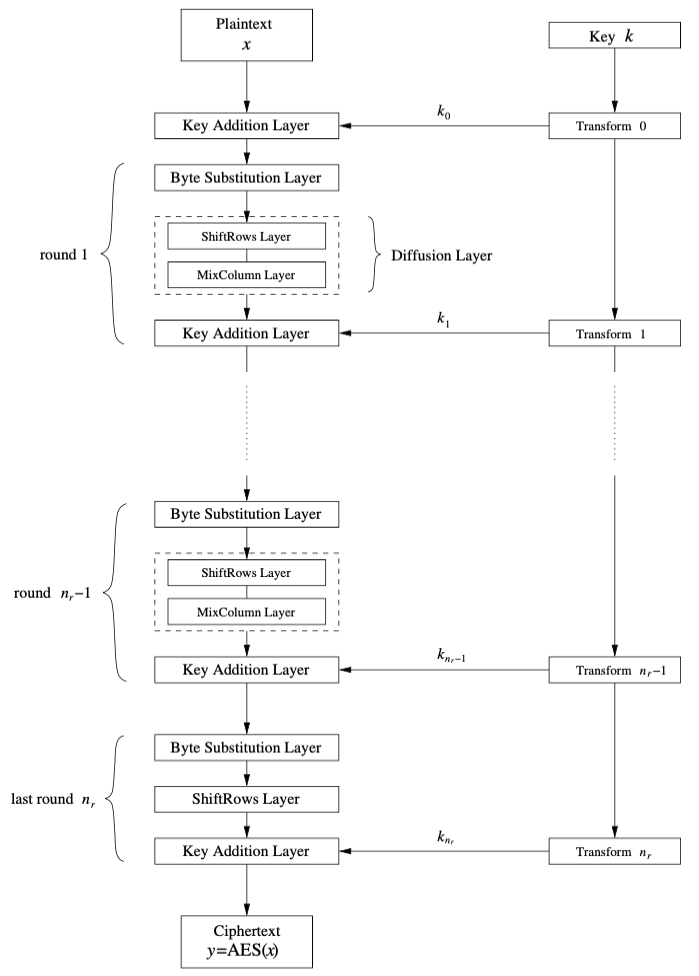
\includegraphics[width=.8\textwidth]{aes-block-diagram.png} % Adjust width as needed
    \caption{
        AES Encryption Block Diagram.
        The plaintext is denoted as $x$, the ciphertext as $y$, key as $k$, and the number of rounds as $n_r$.
    }
    \label{fig:aes-block-diagram} % Reference this figure with \ref{fig:sample_image}
\end{figure}
 


\subsection{Key Size vs. Rounds}

The Rijndeal block and key size vary between 128, 192, and 256 bits.
However, the AES standard calls for a block size of 128 bits. 
The key length directly determines the number of encryption rounds the algorithm performs, as described in 

In AES, the block size is fixed at 128 bits, but the key size can vary between 128, 192, and 256 bits. 
The key length determines the number of rounds used in the encryption process, as outlined in Table \ref{table:key-length-rounds}.

\begin{table}[h]
    \centering
    \begin{tabular}{c|c}
        \textbf{Key length (bit)} & \textbf{\# rounds ($n_r$)} \\ 
        \hline
        128 & 10 \\  
        192 & 12 \\  
        256 & 14 \\  
    \end{tabular}
    \caption{Key lengths and number of rounds for AES}
    \label{table:key-length-rounds}
\end{table}



\subsection{Advantages over DES}

AES offers several advantages over the older DES, particularly in terms of security and efficiency \cite{techtarget_AES_DES}.

\paragraph{Security} 
AES uses a 128-bit block size, compared to DES's 64-bit block size. 
This larger block size significantly enhances security by increasing resistance against brute-force and cryptanalytic attacks. 
% Additionally, AES supports longer key lengths (128, 192, and 256 bits), further improving its cryptographic strength.

\paragraph{Flexibility}
AES supports three different key sizes: 128, 192, and 256 bits, allowing users to choose the level of security they need based on their specific application. 
In contrast, DES uses a fixed 56-bit key, which limits its cryptographic strength. 
Developers can choose from multiple key lengths in AES allows for greater adaptability in meeting varying security requirements.%, especially as computational power increases over time.

\paragraph{Efficiency}
AES processes all 128 bits of data in each round, whereas DES effectively operates on 32 bits per round due to its Feistel structure, which splits the 64-bit block into two halves. 
This allows AES to achieve a higher throughput with fewer computational steps, making it well-suited for both software and hardware implementations.

\section{History of AES}

The history of the Advanced Encryption Standard (AES) reflects a turning point in cryptographic development, 
addressing the weakness of the Data Encryption Standard (DES) and resulting in the selection of Rijndael as the new standard.  

\subsection{Why DES Failed and AES Was Needed}

Initially adopted in the 1970s, DES became one of the most widely used symmetric encryption algorithms. However, by the late 1990s, 
its security was more and more questioned due to its short key length of 56 bits. This key size made DES vulnerable to brute-force attacks, 
as demonstrated by projects like the Electronic Frontier Foundation's DES cracker - \textit{Deep Crack} (shown in Figure~\ref{fig:deep-crack})—which could break DES within days. 
Furthermore, DES was susceptible to various cryptanalytic techniques, including differential and linear cryptanalysis, which exploited its structural weaknesses. 
Although Triple DES (3DES) extended DES's lifespan by using multiple keys, it was computationally inefficient and unsuitable for many modern applications.  
These vulnerabilities not only compromised data integrity but also emphasized the urgent need for a more robust encryption standard that could provide 
better security and efficiency for a wide range of applications. 

\begin{figure}[h] % 'h' means place the figure here if possible
    \centering
    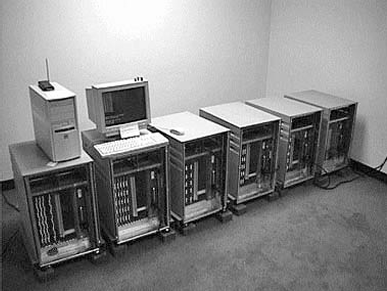
\includegraphics[width=.5\textwidth]{deep_crack.png} % Adjust width as needed
    \caption{
        Deep Crack - the hardware exhaustive key-search machine that broke DES in 1998~\cite{Paar2024}
    }
    \label{fig:deep-crack} % Reference this figure with \ref{fig:sample_image}
\end{figure}
 

\subsection{NIST Competition and Selection Process}

To address the arising challenges, the National Institute of Standards and Technology (NIST) launched a global competition in 1997 to select a new encryption standard. 
The evaluation criteria included security strength, performance across various platforms, flexibility in supporting different key sizes, and resistance to known cryptanalytic attacks. 
After thorough discussion in the scientific community, five finalists—MARS, RC6, Serpent, Twofish, and Rijndael—were selected for further scrutiny. \newline 


Developed by Belgian cryptographers Vincent Rijmen and Joan Daemen, Rijndael was ultimately chosen as the AES algorithm due to its outstanding performance in meeting all evaluation criteria. 
It supports key sizes of 128, 192, and 256 bits while maintaining a fixed block size of 128 bits for AES. NIST officially adopted Rijndael as AES with the publication of 
Federal Information Processing Standards (FIPS) 197 in November 2001. 
\section{AES High Level Structure}

\subsection{What are AES Rounds?}

AES operates on fixed-size blocks of 128 bits, and unlike the DES, it does not use a Feistel structure. 
Instead, AES performs a series of full data transformations, 
which allows it to process the entire 128-bit block in parallel during each round. 
Therefore, it shows the results in fewer rounds; however, the number of rounds depends on the key size.
\noindent
Each AES round consists of a layered structure where the internal state 
- represented as a four-by-four-byte matrix - is progressively manipulated. 
The full AES encryption process is divided into three main phases: the initial round, 
a set of main rounds, and a final round.
\noindent
The design of these rounds ensures symmetry between encryption and decryption, 
particularly due to the final round omitting the \texttt{MixColumns} transformation. 
This allows the inverse operations used during decryption to align correctly with the forward structure used in encryption.

\subsection{The Initial Round}

The initial round works through a single operation called \texttt{AddRoundKey}; in this step, 
the 128-bit plaintext block is organised into a four-by-four matrix, the state. 
Each byte of the state is combined using an XOR operation with a corresponding byte from the first-round key. 
This round key is derived from the original AES key using the key expansion process.
\noindent
Through this step, the key blends with the data from the beginning and adds an initial confusion layer, 
preparing the state for the transformations that will occur in the following rounds. 
This round does not involve any substitution or shifting steps; nevertheless, these will begin with the main rounds.

\subsection{Main Rounds}

Each main round applies the following four transformations in order:

\begin{enumerate}
    \item \textbf{SubBytes} – a nonlinear substitution step where each byte in the state is replaced through an S-box, 
    introducing non-linearity and confusion.
    \item \textbf{ShiftRows} – a permutation step that shifts the bytes in each 
    row of the state to the left by a certain number of positions, increasing diffusion.
    \item \textbf{MixColumns} – a mixing transformation that combines the bytes in each column using 
    matrix multiplication over a Galois Field, spreading the influence of each byte throughout the state.
    \item \textbf{AddRoundKey} – the updated round key is applied to the current state using the XOR operation.
\end{enumerate}
\noindent
These layers together ensure that each round produces a progressively more complex output, 
significantly transforming the state from the original input with each iteration.

\subsection{Final Round}
\noindent
The final round is similar to the main rounds, but it omits the \texttt{MixColumns} step. 
This minor simplification maintains symmetry in AES, 
allowing the decryption process to correctly reverse the encryption steps, 
as \texttt{MixColumns} is not naturally invertible.

\section{Internal Structure of AES}

\begin{figure}[h] % 'h' means place the figure here if possible
    \centering
    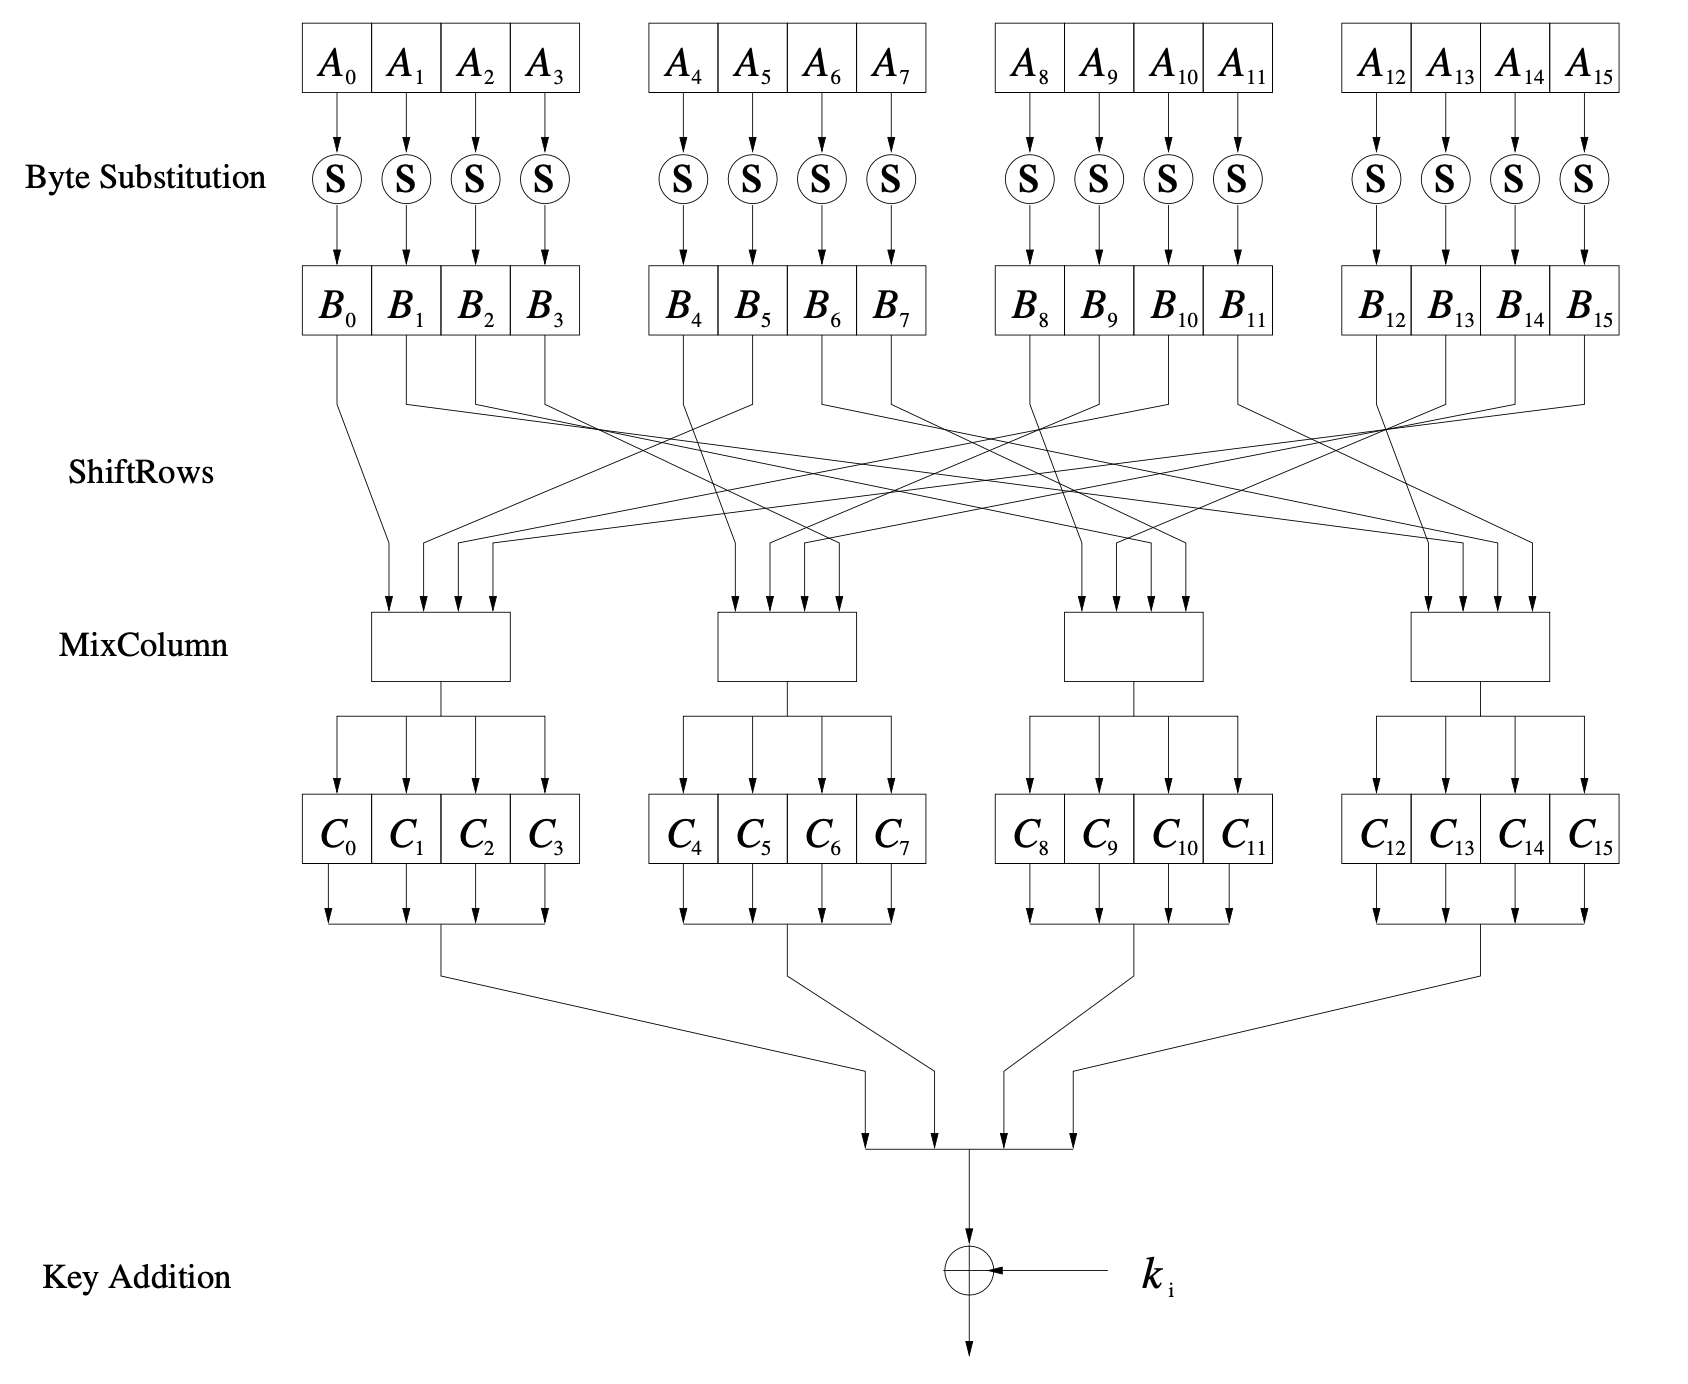
\includegraphics[width=.8\textwidth]{aes-round-function.png} % Adjust width as needed
    \caption{
        AES round function for rounds $1, 2, \dots, n_r-1$.
    }
    \label{fig:aes-round-function} % Reference this figure with \ref{fig:sample_image}
\end{figure}

Figure \ref{fig:aes-round-function} shows the graph of a single AES round. 
The 16-byte input $A_0, \dots, A_{15}$ is fed byte-wise into the S-Box in the Byte Substitution Layer (Section \ref{sec:byte-substitution}).
The 16-byte output $B_0, \dots, B_{15}$ is permutated twice in the \texttt{ShiftRows} layer and mixed by the \texttt{MixColumn} transformation, both in the Diffusion layer (Section \ref{sec:diffusion})
Finally, the 128-bit subkey $k_i$ is XORed with the immediate result in the Key Addition layer (Section \ref{sec:key-addition}).


% \subsection{Byte Substitution Layer}
\label{sec:byte-substitution}



\subsection{Diffusion Layer}
\label{sec:diffusion}

The diffusion spreads the influence of individual bits over the entire state, and spreads the influence of individual bits over the entire state.
The diffusion layer consists of two sublayers: the \texttt{ShiftRows} transformation and the \texttt{MixColumn} transformation.


\subsubsection{\texttt{ShiftRows} Sublayer}

The \texttt{ShiftRows} transformation cyclincally shifts the second row of the state matrix three bytes to the right, the third row by two bytes to the right, and the forth row by one byte to the right.
The first row is not changed.

The purpose of this is to increase the diffusion properties of AES.

% \[
% \begin{align}
%   &\begin{array}{|c|c|}
%     \hline
%     ID & Name \\
%     \hline
%     1 & Alice \\
%     2 & Bob \\
%     \hline
%   \end{array}
%   \quad \longrightarrow \quad
%   \begin{array}{|c|c|}
%     \hline
%     ID & Score \\
%     \hline
%     1 & 85 \\
%     2 & 92 \\
%     \hline
%   \end{array}
% \end{align}
% \]

\begin{equation}
    \begin{array}{c@{\quad \longrightarrow \quad}c}
        \begin{array}{|c|c|c|c|}
        \hline
        B_0 & B_4 & B_8 & B_{12} \\
        \hline
        B_1 & B_5 & B_9 & B_{13} \\
        \hline
        B_2 & B_6 & B_{10} & B_{14} \\
        \hline
        B_3 & B_7 & B_{11} & B_{15} \\
        \hline
        \end{array}
    &
    \begin{array}{|c|c|c|c|}
        \hline
        B_0 & B_4 & B_8 & B_{12} \\
        \hline
        B_5 & B_9 & B_{13} & B_1 \\
        \hline
        B_{10} & B_{14} & B_2 & B_6 \\
        \hline
        B_{15} & B_3 & B_7 & B_{11} \\
        \hline
        \end{array}
    \end{array}
\end{equation}





\subsubsection{\texttt{MixColumn} Sublayer}

The \texttt{MixColumn} transformation is a linear transformation which mixes each column of the state matrix. 
\begin{align}
    MixColumn(B) &= C\\
    \begin{pmatrix}
        02 & 03 & 01 & 01\\
        01 & 02 & 03 & 01\\
        01 & 01 & 02 & 03\\
        03 & 01 & 01 & 02
    \end{pmatrix}
    \cdot
    \begin{pmatrix}
        B_0 & B_4 & B_8 & B_{12} \\
        B_5 & B_9 & B_{13} & B_1 \\
        B_{10} & B_{14} & B_2 & B_6 \\
        B_{15} & B_3 & B_7 & B_{11} \\
    \end{pmatrix}
    &=
    \begin{pmatrix}
        C_0 & C_4 & C_8 & C_{12} \\
        C_1 & C_5 & C_9 & C_{13} \\
        C_2 & C_6 & C_{10} & C_{14} \\
        C_3 & C_7 & C_{11} & C_{15} \\
    \end{pmatrix}
\end{align}
with $B$ being the 16-byte input state after \texttt{ShiftRows} operation given in Equation \ref{} and C being the 16-byte output state.
Each vector column of B is multiplied by a fixed $4 \times 4$ matrix (containing constant entries).


\subsection{Key Addition Layer}
\label{sec:key-addition}


\section{Key Expansion}

\subsection{Importance of Key Expansion in AES} 

The Advanced Encryption Standard (AES) heavily relies on the key expansion (or key schedule), 
a process that derives a series of round keys from the initial cipher key. 
This process ensures that each round uses a different key, 
greatly increasing the cipher's security. The key expansion process slightly differs 
based on the AES version (AES-128, AES-192, or AES-256), mainly in the number of rounds 
and the size of the key.

\subsection{Main Algorithm of Key Expansion}

First, the initial key is loaded into the first $N_k$ words of the key schedule, where $N_k$ depends 
on the key size $K_{len}$ and the number of rounds $N_r$: ($K_{len}$, $N_r$) = (128, 10), (192, 12), and (256, 14) 
for AES-128, AES-192, and AES-256, respectively \cite{Key_Collisions} (shown in Figure~\ref{fig:key_comb}). AES requires $N_r+1$ round keys, each round key is 
128 bits (16 bytes) in size, equivalent to four words $N_b$ from the key schedule. The key schedule in 
response generates a total of $N_b$×($N_r+1$) words\cite{Standards2001}. \newline

For example, for AES-192, the key schedule generates 52 words in the key expansion, which equals 208 bytes (4 \textit{bytes per word} × 52 \textit{words}).
13 round keys are then extracted from these words - one for each of the 12 rounds plus the initial key addition ($N_r$ + 1 = 13).

\begin{figure}[h] % 'h' means place the figure here if possible
    \centering
    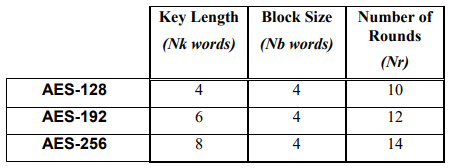
\includegraphics[width=.8\textwidth]{197_key_combinations.png} % Adjust width as needed
    \caption{
        Key-Block-Round Combinations \cite{Standards2001}
    }
    \label{fig:key_comb} % Reference this figure with \ref{fig:sample_image}
\end{figure}

Then, the remaining words are generated iteratively. For words at positions that are a multiple of $N_k$, a 
transformation is applied to the previous word w[i-1] before the XOR. This transformation consists of RotWord 
followed by SubWord, and the result is then XORed with a round constant Rcon[i], where:

\begin{enumerate}
    \item \textbf{RotWord}: A cyclic permutation that shifts the bytes in the 4-byte input word one position to the left. 
    \item \textbf{SubWord}: A substitution operation that applies SubBytes operation to a 4-byte input word. 
    \item \textbf{Round Constant (Rcon)}:  An XOR operation with a round-dependent constant RC, where each Rcon[i]
    has a structure (RC[i], 0x00, 0x00, 0x00) \cite{Standards2001}. 
\end{enumerate}

If the AES version is AES-256 ($N_k$ = 8) and i-4 is a multiple of $N_k$, the SubWord transformation is applied to the 
previous word (shown in Figure), but RotWord and Rcon are skipped. Otherwise, the new word is generated by XORing the previous word 
with the word $N_k$ positions earlier in the key schedule \cite{Standards2001}. 

\begin{figure}[h] % 'h' means place the figure here if possible
    \centering
    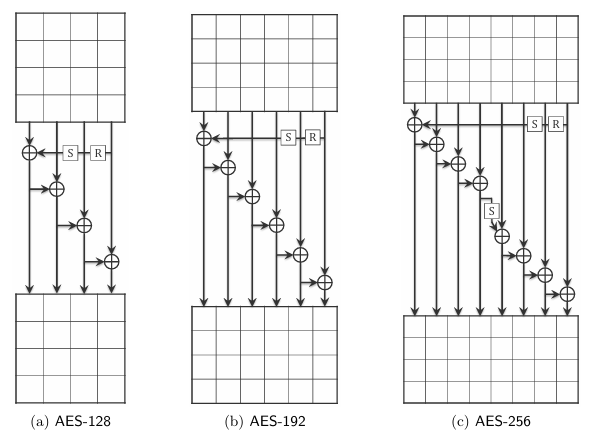
\includegraphics[width=.8\textwidth]{key_schedules.png} % Adjust width as needed
    \caption{
        Key schedules of AES-128, AES-192, and AES-256.The SubWord and
        RotWord functions are denoted by $S$ and $R$, respectively. Note that the round
        constant is not shown. \cite{Key_Collisions}
    }
    \label{fig:key_comb} % Reference this figure with \ref{fig:sample_image}
\end{figure}

\subsection{Key Size and Security}

The key size directly impacts the security level of the algorithm, with 
longer keys providing higher security against brute force attacks. AES-128 offers sufficient security 
for most applications, but AES-192 and AES-256 are often preferred for applications requiring 
long-term security or protecting highly sensitive data. The increased number of rounds in AES-256 
further enhances its resistance against advanced cryptanalytic techniques.

\subsection{Innovative Key Generation Methods}

Researchers continue to explore alternative key generation methods to enhance security or efficiency. 
The Sudoku-AES algorithm enhances cryptographic security by integrating Sudoku puzzle mechanics into 
the AES's key generation and expansion phases. This approach replaces Rijndael's static key schedule 
with dynamic key pools derived from Sudoku matrices, improving the cipher's resistance  to 
brute-force and side-channel attacks. \cite{Sudoku_Method}

\subsubsection{Main Algorithm - Sudoku Maxtix Construction}

Partially filled 9×9 Sudoku grid is created following the 
games rules - no duplicates in rows/columns/3×3 subgrids. The numbers 1 to 9 from the solved 9×9 KeyMatrix 
are converted to equivalent hexadecimal 4×9 KeyPool matrix as shown in Figure~\ref{fig:sudoku}. During encryption, 
keys of appropriate length (128/192/256 bits) are celected from this pool. \cite{Sudoku_Method}

\begin{figure}[h] % 'h' means place the figure here if possible
    \centering
    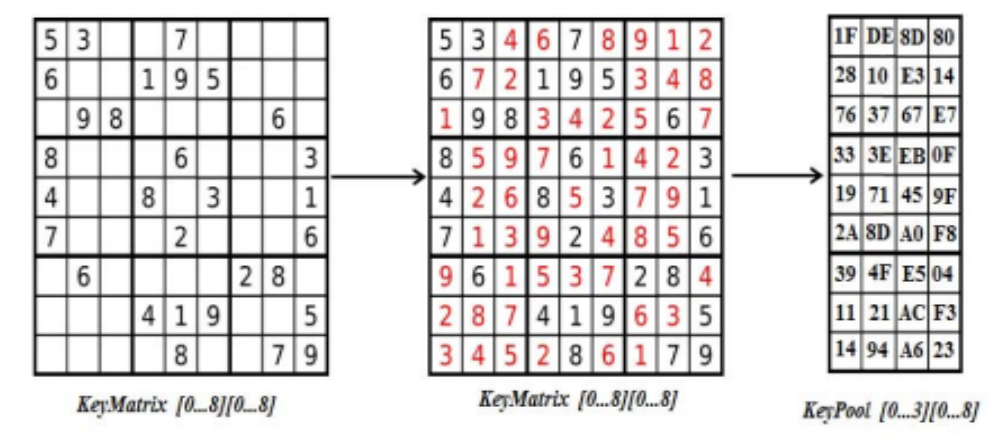
\includegraphics[width=.8\textwidth]{sudoku.png} % Adjust width as needed
    \caption{
        Key Pool Generation \cite{Sudoku_Method}
    }
    \label{fig:sudoku} % Reference this figure with \ref{fig:sample_image}
\end{figure}

\subsubsection{Advantages of Sudoku Method}

The strength of this method lies in the difficulty of predicting the Sudoku solution, which provides 
a unique key pool for each user. It requires minimum execution time compare to other similar algorithms, 
with the time complexity of KeyPool generation O(($n^2$)!), making it both fast and efficient. \cite{Sudoku_Method} 

\input{content/different-aes-version.tex}
% \section{Security Analysis}

\subsection{Why AES is Considered Secure?}

\subsection{Known Attacks on AES}

\subsection{Why These Attacks are Hard to Pull Off?}
\section{AES Modes of Operation}

\subsection{What are Modes of Operation?}

Block ciphers such as AES are designed to encrypt fixed-length blocks (e.g., 128 bits), 
but real-world applications typically require secure encryption of variable-length messages. 
Modes of operation define how to securely encrypt these longer messages by specifying how individual blocks are chained or transformed during encryption. 
They significantly influence the security and efficiency of the cipher and must be selected carefully based on application requirements.

\subsection{Electronic Codebook (ECB) Mode}

ECB is the simplest AES mode where each plaintext block is encrypted independently:
\[
y_i = E_k(x_i), \quad x_i = D_k(y_i)
\]
Its determinism leads to serious vulnerabilities: identical plaintext blocks produce identical ciphertexts. 
This exposes structural patterns in the plaintext, making it unsuitable for most practical applications.

\subsection{Cipher Block Chaining (CBC) Mode}

CBC introduces chaining by XORing each plaintext block with the previous ciphertext:
\[
\begin{aligned}
y_1 &= E_k(x_1 \oplus IV) \\
y_i &= E_k(x_i \oplus y_{i-1}) \\
x_1 &= D_k(y_1) \oplus IV \\
x_i &= D_k(y_i) \oplus y_{i-1}
\end{aligned}
\]
A random initialisation vector (IV) ensures semantic security. 
However, CBC decryption is parallelisable, while encryption is inherently sequential.

\subsection{Cipher Feedback (CFB) Mode}

CFB operates as a self-synchronising stream cipher:
\[
\begin{aligned}
s_1 &= E_k(IV), \quad y_1 = x_1 \oplus s_1 \\
s_i &= E_k(y_{i-1}), \quad y_i = x_i \oplus s_i
\end{aligned}
\]
This mode provides partial error recovery and supports smaller data units, such as bytes.

\subsection{Output Feedback (OFB) Mode}

OFB, like CFB, transforms AES into a stream cipher, but the key stream is independent of the ciphertext:
\[
\begin{aligned}
s_1 &= E_k(IV), \quad y_1 = x_1 \oplus s_1 \\
s_i &= E_k(s_{i-1}), \quad y_i = x_i \oplus s_i
\end{aligned}
\]
It offers full error isolation, but loss of synchronisation between sender and receiver leads to complete decryption failure.

\subsection{Counter (CTR) Mode}

CTR mode generates a keystream using an incrementing counter:
\[
y_i = x_i \oplus E_k(\text{Nonce} || \text{CTR}_i)
\]
It supports full parallelisation and random access to encrypted data, making it highly suitable for high-throughput systems.

\subsection{XTS-AES: A Mode for Disk Encryption}

XTS-AES was developed specifically for encrypting data on storage devices. 
It employs a tweakable block cipher and uses two keys, $k_1$ and $k_2$, 
to compute a unique tweak $T$ for each data block:

\[
\begin{aligned}
T &= E_{k_2}(i) \cdot \alpha^j \\
y_j &= E_{k_1}(x_j \oplus T) \oplus T
\end{aligned}
\]

This structure ensures that identical plaintext blocks at different locations produce different ciphertexts, and supports efficient parallel processing.

\subsection{Post-Quantum Security and AES Modes of Operation}

The development of quantum computing poses significant threats to symmetric-key ciphers via Grover’s algorithm, 
which reduces brute-force complexity from $2^k$ to about $2^{k/2}$. 

\noindent As such, AES-128 may offer only $2^{64}$ bits of effective quantum security.
Recent work by Jang et al.~\cite{Jang2025} improves resource estimation for quantum AES implementations using optimised Grover’s circuits. \newline

\noindent Their findings yield the following security estimates:
\begin{itemize}
    \item AES-128: $2^{156.26}$
    \item AES-192: $2^{221.58}$
    \item AES-256: $2^{286.07}$
\end{itemize}

The study also introduces low-depth circuit architectures designed to comply with NIST’s \texttt{MAXDEPTH} constraint, 
emphasising modes that support parallelism.

\textbf{Mode Implications:}
\begin{itemize}
    \item \textbf{ECB:} Highly insecure; reveals structure under both classical and quantum analysis.
    \item \textbf{CBC:} Limited parallelism; not ideal in depth-constrained quantum models.
    \item \textbf{CFB/OFB:} Less deterministic; may provide robustness depending on IV usage.
    \item \textbf{CTR:} Well-suited for quantum-resilient designs due to full parallelism.
    \item \textbf{XTS:} Offers random block access and tweakable security; strong candidate for post-quantum storage encryption.
\end{itemize}

\subsection{Summary of Modes of Operation}

\begin{table}[h]
\centering
\begin{tabular}{|l|c|c|c|l|}
\hline
\textbf{Mode} & \textbf{Parallel} & \textbf{Error Prop.} & \textbf{Random Access} & \textbf{Best For} \\
\hline
ECB & Yes & None & Yes & Testing, toy cases \\
CBC & No (Enc) / Yes (Dec) & Next block & No & File encryption \\
CFB & No & Next block & No & Streaming with feedback \\
OFB & Yes & None & No & Error-resilient streaming \\
CTR & Yes & None & Yes & High-speed applications \\
XTS & Yes & None & Yes & Disk encryption \\
\hline
\end{tabular}
\caption{Comparison of AES modes of operation.}
\end{table}

\section{Applications of AES Encryption in Real World}

\subsection{Wireless Security (Wi-Fi)}
\Gls{AES} is commonly used together with Wi-Fi security protocols (such as WPA2 and WPA3) to encrypt data transmitted over wireless networks.
This is to ensure that sensitive information, like passwords and personal data, remains protected from unauthorised access \cite{cooper2025aes}.


\subsection{Encrypted Browsing (HTMLS)}
Websites use \gls{AES} encryption within HTTPS protocols to ensure data transmitted between browsers and servers.
This encryption helps protect user information, such as login credentials and payment details, from interception by malicious actors \cite{cooper2025aes}.


\subsection{Virtual Private Networks}
The job of a \gls{VPN} is to securely connect user to another server online, only the best encryption can be considered so that the user's data will not be leaked.
The \glspl{VPN} that use \gls{AES} with 256-bit keys include NordVPN, Surfshark, and ExpressVPN \cite{rimkiene2022aes}.


\subsection{File and Disk Encryption}
Operating systems like Windows and macOS offer \gls{AES}-based encryption options (e.g. BitLocker and FileVault) for securing entire hard drives or individual files.
This is particularly useful for safeguarding personal or sensitive business information stored on physical devices \cite{cooper2025aes}.


\subsection{Cloud Storage}
\Gls{AES} encryption is essential for securing files stored in cloud environments.
Services like Google Drive, Dropbox, and others use \gls{AES} to ensure that uploaded files remain confidential and protect against unauthorised access \cite{cooper2025aes}.


\subsection{Mobile Applications}
Many mobile apps, especially those dealing with financial transactions or personal data, use \gls{AES} encryption to secure data on devices and in transit.
This includes banking apps, social media platforms, and messaging apps, providing users with a piece of mind that their data is protected \cite{cooper2025aes}.


\subsection{Secure Messaging}
Many encrypted messaging applications, like Signal and WhatsApp, use \gls{AES} to secure messages end-to-end, ensuring that only the sender and recipient can read contents of their conversations \cite{cooper2025aes}.


\subsection{Password Managers}
These are the programs that carry a lot of sensitive information.
Hence, password managers like LastPass and Dashlane include the important step of \gls{AES} implementation \cite{rimkiene2022aes}.



% \appendix
% \section{Appendix}

\lstinputlisting[
    caption={Implementation of the \gls{AES} algorithm},
    label={lst:aes-impl}
]{code/aes.py}

\lstinputlisting[
    caption={Bitwise operations for finite field arithmetic},
    label={lst:bin-math}
]{code/bin_math.py}

\lstinputlisting[
    caption={Helper functions for \gls{AES} operations},
    label={lst:fxns}
]{code/functions.py}



\newpage
\printbibliography


\end{document}